\section{Introduction}

Transformers-based model is the latest state-of-the-art model in machine learning approach of natural language processing. From the observation in Figure~\ref{fig:bert_benchmark}, increasing the number of GPUs does reduce the training time, but the speed-up factor is fairly low when reaching 4 GPUs. In order to inspect the root cause, we profile the activities of multi-GPUs and a single GPU for fine-tuning WangchanBERTa, a Deep Learning model on a Thai corpus for classification task as well as GPT-2 to benchmark a downstream task. The objective is to test the scalability and runtime of each function by tracing the calling of CUDA operators via NVProf.

\begin{figure}[h!]
    \centering
    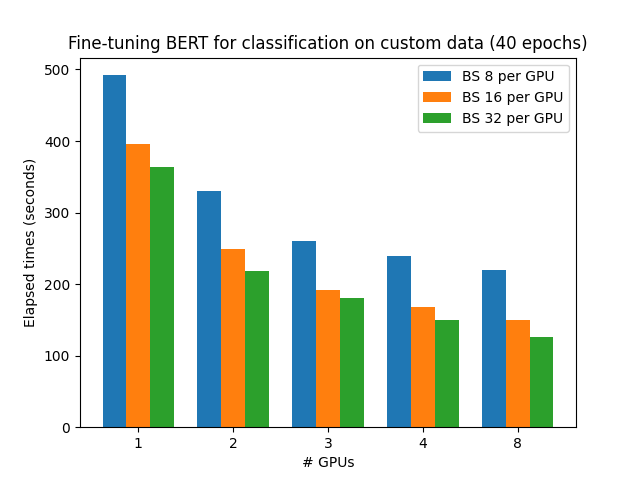
\includegraphics[width=0.7\columnwidth]{fig/benchmark_bybs_1.png}
    \caption{Wall clock time of fine-tuning BERT on various number of graphic cards on DGX}
    \label{fig:bert_benchmark}
\end{figure}


% \noindent\textbf{Subheading.} is a sample of how you can use a bold text without indentation. This
% technique can be handy if you want to stress the key topic that is going to be discussed in this
% paragraph. Example below.

% \noindent\textbf{Our goal.} The goal of this template is threefold. First, I want to make sure that
% everyone gets familiar with LaTeX, which is a very handy everyone should use when writing papers.

 
 

% \blfootnote{The repository URL: \url{https://github.com/calzonelover/Profiling-Transformer-Based-Model}}
